% ============================================================
\chapter{Introduction to PDEs}
\label{ch:introduction}
% ============================================================

Partial differential equations are the language in which nature writes its
laws. The heat equation describes how temperature diffuses through metal.
The wave equation governs a vibrating guitar string, the propagation of
sound, and the gravitational waves predicted by Einstein. Laplace's equation
reigns over electrostatics, Newtonian gravity, and incompressible fluid
flow. Schr\"odinger's equation determines the evolution of every quantum
system.

These equations, discovered over three centuries by Euler, d'Alembert,
Fourier, Laplace, and many others, share a common characteristic: they
relate an unknown function of several variables to its partial derivatives.
They are richer --- and harder --- than ordinary differential equations,
because the multiplicity of space and time variables engenders a variety of
behaviors: diffusion, propagation, equilibrium. This first chapter maps out
this territory.

% ------------------------------------------------------------
\section{What is a PDE?}
% ------------------------------------------------------------

Let us begin with the most general definition, before specializing.

\begin{definition}[Partial differential equation]
A \textbf{partial differential equation} (PDE) is an equation involving an
unknown function $u$ of several independent variables
$(x_1, \ldots, x_n)$ and its partial derivatives. The general form is:
\[
    F\bigl(x_1, \ldots, x_n, u, u_{x_1}, \ldots, u_{x_n},
    u_{x_1 x_1}, u_{x_1 x_2}, \ldots\bigr) = 0.
\]
\end{definition}

\begin{definition}[Order of a PDE]
The \textbf{order} of a PDE is the highest order of partial differentiation
appearing in the equation.
\end{definition}

\begin{example}
Some classical PDEs:
\begin{enumerate}
    \item \textbf{Transport equation} (order 1): $u_t + c\, u_x = 0$.
    \item \textbf{Heat equation} (order 2): $u_t = k\, u_{xx}$.
    \item \textbf{Wave equation} (order 2): $u_{tt} = c^2 u_{xx}$.
    \item \textbf{Laplace equation} (order 2): $\Delta u = 0$.
    \item \textbf{Burgers' equation} (order 1, nonlinear):
          $u_t + u\, u_x = 0$.
    \item \textbf{Korteweg--de Vries equation} (order 3):
          $u_t + 6u\, u_x + u_{xxx} = 0$.
\end{enumerate}
\end{example}

\section{Linearity and homogeneity}

\begin{definition}[Linear PDE]
A PDE is \textbf{linear} if the operator $L$ defined by the left-hand side
is linear, i.e.,
\[
    L(\alpha u + \beta v) = \alpha\, L(u) + \beta\, L(v)
    \quad \forall \alpha, \beta \in \R.
\]
The PDE is \textbf{homogeneous} if $Lu = 0$, and \textbf{inhomogeneous} if
$Lu = f$ with $f \neq 0$.
\end{definition}

\begin{remark}
The \textbf{superposition principle} applies to linear homogeneous PDEs:
if $u_1$ and $u_2$ are solutions, then $\alpha u_1 + \beta u_2$ is also a
solution for all $\alpha, \beta \in \R$. This principle is fundamental for
the method of separation of variables.
\end{remark}

\begin{definition}[Semilinear, quasilinear, fully nonlinear]
\leavevmode
\begin{itemize}
    \item \textbf{Semilinear}: linear in the highest-order derivatives, with
          coefficients depending only on $x$:
          $\Delta u = f(x, u, \nabla u)$.
    \item \textbf{Quasilinear}: linear in the highest-order derivatives, with
          coefficients depending on $u$ and $\nabla u$:
          $\sum a_{ij}(x, u, \nabla u)\, u_{x_i x_j} = f(x, u, \nabla u)$.
    \item \textbf{Fully nonlinear}: nonlinear in the highest-order
          derivatives: $\det(D^2 u) = f$ (Monge--Amp\`ere equation).
\end{itemize}
\end{definition}

\section{Classification of second-order PDEs}

Consider a second-order PDE in two independent variables:
\begin{equation}\label{eq:second_order_pde}
    a(x,y)\, u_{xx} + 2b(x,y)\, u_{xy} + c(x,y)\, u_{yy}
    + d(x,y)\, u_x + e(x,y)\, u_y + f(x,y)\, u = g(x,y).
\end{equation}

\begin{definition}[Classification by discriminant]
The \textbf{discriminant} of the PDE \eqref{eq:second_order_pde} is
$\Delta_{\mathrm{disc}} = b^2 - ac$. The PDE is said to be:
\begin{itemize}
    \item \textbf{Elliptic} if $b^2 - ac < 0$ at every point of the domain.
    \item \textbf{Parabolic} if $b^2 - ac = 0$ at every point of the domain.
    \item \textbf{Hyperbolic} if $b^2 - ac > 0$ at every point of the domain.
\end{itemize}
\end{definition}

\begin{intuition}
This classification has deep physical meaning:
\begin{itemize}
    \item \textbf{Elliptic} PDEs (Laplace type) model equilibrium states:
          the solution at a point depends on the solution everywhere around it.
    \item \textbf{Parabolic} PDEs (heat type) model diffusion processes:
          information propagates at infinite speed but attenuates.
    \item \textbf{Hyperbolic} PDEs (wave type) model propagation phenomena:
          information travels at finite speed along characteristics.
\end{itemize}
\end{intuition}

\begin{example}
\leavevmode
\begin{enumerate}
    \item $u_{xx} + u_{yy} = 0$ (Laplace): $a = 1$, $b = 0$, $c = 1$,
          so $b^2 - ac = -1 < 0$: \textbf{elliptic}.
    \item $u_t - u_{xx} = 0$ (heat): $a = -1$, $b = 0$, $c = 0$,
          so $b^2 - ac = 0$: \textbf{parabolic}.
    \item $u_{tt} - c^2 u_{xx} = 0$ (wave): $a = -c^2$, $b = 0$, $c_{\text{coeff}} = 1$,
          so $b^2 - ac = c^2 > 0$: \textbf{hyperbolic}.
\end{enumerate}
\end{example}

\subsection{Classification in higher dimensions}

For a second-order PDE in $n$ variables:
\[
    \sum_{i,j=1}^{n} a_{ij}(x)\, u_{x_i x_j}
    + \text{lower-order terms} = 0,
\]
the classification is based on the \textbf{coefficient matrix}
$A = (a_{ij})$, assumed symmetric:
\begin{itemize}
    \item \textbf{Elliptic}: all eigenvalues of $A$ have the same sign.
    \item \textbf{Hyperbolic}: one eigenvalue has opposite sign to the others.
    \item \textbf{Parabolic}: one zero eigenvalue, the rest having the same sign.
\end{itemize}

\begin{theorem}[Canonical form --- case $n=2$]
By a suitable change of variables $(\xi, \eta) = (\xi(x,y), \eta(x,y))$,
every linear second-order PDE in two variables can be reduced to one of
the following canonical forms:
\begin{itemize}
    \item \textbf{Elliptic}: $u_{\xi\xi} + u_{\eta\eta} + \cdots = 0$.
    \item \textbf{Parabolic}: $u_{\xi\xi} + \cdots = 0$.
    \item \textbf{Hyperbolic}: $u_{\xi\xi} - u_{\eta\eta} + \cdots = 0$
          or equivalently $u_{\alpha\beta} + \cdots = 0$ with
          $\alpha = \xi + \eta$, $\beta = \xi - \eta$.
\end{itemize}
\end{theorem}

\section{Boundary conditions and initial conditions}

\begin{definition}[Boundary value problem]
A \textbf{boundary value problem} consists of a PDE posed on a domain
$\Omega \subset \R^n$ supplemented with conditions on the boundary
$\partial\Omega$. The main types are:
\begin{enumerate}
    \item \textbf{Dirichlet}: $u = g$ on $\partial\Omega$.
    \item \textbf{Neumann}: $\frac{\partial u}{\partial \nu} = g$ on
          $\partial\Omega$, where $\nu$ is the outward unit normal.
    \item \textbf{Robin} (mixed): $\alpha u + \beta \frac{\partial u}{\partial \nu} = g$
          on $\partial\Omega$.
\end{enumerate}
\end{definition}

\begin{center}
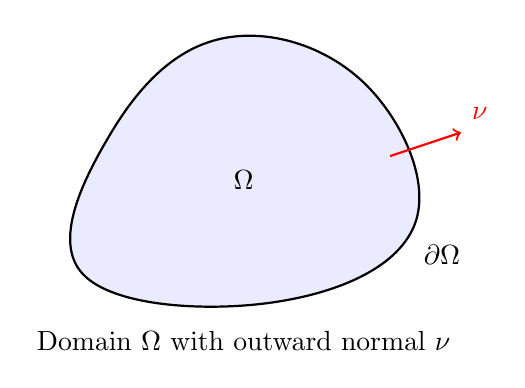
\begin{tikzpicture}[scale=1.2]
    % Domain
    \draw[thick, fill=blue!8] plot[smooth cycle, tension=0.7]
        coordinates {(0,0) (2,-0.3) (3.5,0.5) (3,2) (1.5,2.5) (0.3,1.5)};
    \node at (1.7,1) {$\Omega$};
    % Normal
    \draw[->, thick, red] (3.25,1.25) -- (4.0,1.5);
    \node[red] at (4.2,1.7) {$\nu$};
    % Labels
    \node at (3.8,0.2) {$\partial\Omega$};
    \node[below] at (1.7, -0.5) {Domain $\Omega$ with outward normal $\nu$};
\end{tikzpicture}
\end{center}

\begin{definition}[Well-posed problem in the sense of Hadamard]
A problem is said to be \textbf{well-posed} in the sense of Hadamard if it
satisfies the following three conditions:
\begin{enumerate}
    \item \textbf{Existence}: there exists at least one solution.
    \item \textbf{Uniqueness}: there exists at most one solution.
    \item \textbf{Stability}: the solution depends continuously on the data.
\end{enumerate}
\end{definition}

\begin{warning}[title=\textbf{Importance of well-posedness}]
An ill-posed problem is not necessarily without mathematical or physical
interest. Hadamard's classical example shows that the Cauchy problem for
Laplace's equation is ill-posed, but regularization techniques allow one
to address it.
\end{warning}

\begin{example}[Dirichlet problem for the Laplacian on the disk]
Find $u$ harmonic in the unit disk $D = \{(x,y) : x^2+y^2 < 1\}$
with $u = g$ on $\partial D = \{x^2+y^2=1\}$. In polar coordinates:
\[
    \begin{cases}
        u_{rr} + \frac{1}{r}u_r + \frac{1}{r^2}u_{\theta\theta} = 0,
        & 0 < r < 1,\\
        u(1,\theta) = g(\theta).
    \end{cases}
\]
This problem is well-posed (existence, uniqueness, stability).
\end{example}

\section{Evolution problems}

\begin{definition}[Cauchy problem]
For an evolution PDE (parabolic or hyperbolic), the \textbf{Cauchy problem}
consists of finding $u(x,t)$ satisfying the PDE for $t > 0$ together with
\textbf{initial conditions} at $t = 0$:
\begin{itemize}
    \item For the heat equation: $u(x,0) = u_0(x)$.
    \item For the wave equation: $u(x,0) = u_0(x)$ and $u_t(x,0) = v_0(x)$.
\end{itemize}
\end{definition}

\begin{center}
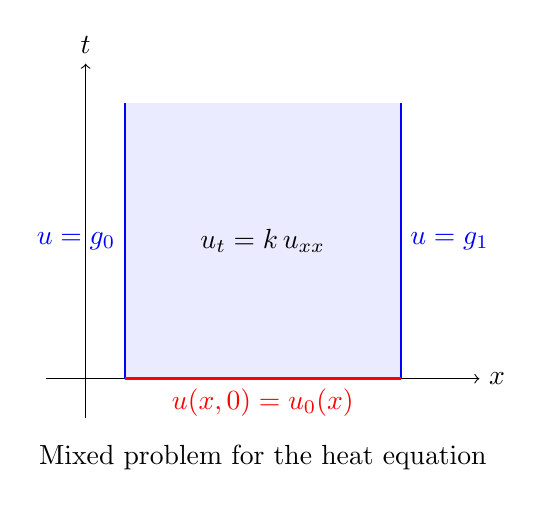
\begin{tikzpicture}[scale=1.0]
    % Axes
    \draw[->] (-0.5,0) -- (5,0) node[right] {$x$};
    \draw[->] (0,-0.5) -- (0,4) node[above] {$t$};
    % Space-time domain
    \fill[blue!8] (0.5,0) rectangle (4,3.5);
    \draw[thick, blue] (0.5,0) -- (0.5,3.5);
    \draw[thick, blue] (4,0) -- (4,3.5);
    \draw[very thick, red] (0.5,0) -- (4,0);
    % Labels
    \node[red, below] at (2.25,0) {$u(x,0) = u_0(x)$};
    \node[blue, left] at (0.5,1.75) {$u=g_0$};
    \node[blue, right] at (4,1.75) {$u=g_1$};
    \node at (2.25,1.75) {$u_t = k\,u_{xx}$};
    \node at (2.25, -1) {Mixed problem for the heat equation};
\end{tikzpicture}
\end{center}

\section{Fundamental modelling examples}

\subsection{Derivation of the heat equation}

Consider a thin rod of length $L$. Let $u(x,t)$ be the temperature at
point $x \in [0,L]$ at time $t$. Energy conservation on a segment $[a,b]$
gives:
\[
    \frac{d}{dt}\int_a^b \rho\, c_p\, u(x,t)\,dx
    = -q(a,t) + q(b,t) + \int_a^b f(x,t)\,dx,
\]
where $\rho$ is the density, $c_p$ the heat capacity, $q$ the heat flux,
and $f$ a source term. Fourier's law gives $q(x,t) = -k\, u_x(x,t)$.
Differentiating under the integral sign:
\[
    \int_a^b \rho\, c_p\, u_t\, dx = \int_a^b k\, u_{xx}\, dx
    + \int_a^b f\, dx.
\]
Since this holds for all $[a,b]$, we obtain:
\[
    \rho\, c_p\, u_t = k\, u_{xx} + f,
\]
and setting $\kappa = k/(\rho c_p)$:
\begin{equation}\label{eq:heat_derivation}
    u_t = \kappa\, u_{xx} + \tilde{f}.
\end{equation}

\subsection{Derivation of the wave equation}

Consider a vibrating string of linear density $\rho$ under tension $T$.
For small transverse displacements $u(x,t)$, Newton's second law applied
to an element $[x, x+dx]$ gives:
\[
    \rho\, dx\, u_{tt} = T\sin\theta(x+dx) - T\sin\theta(x)
    \approx T\bigl(u_x(x+dx) - u_x(x)\bigr) = T\, u_{xx}\, dx.
\]
Hence:
\begin{equation}\label{eq:wave_derivation}
    u_{tt} = c^2\, u_{xx}, \quad c = \sqrt{T/\rho}.
\end{equation}

\section{Examples of explicit solutions}

\begin{example}[Solutions of Laplace's equation in 2D]
The following harmonic functions solve $\Delta u = 0$ in $\R^2$:
\begin{enumerate}
    \item $u(x,y) = ax + by + c$ (affine functions).
    \item $u(x,y) = x^2 - y^2$ (check: $u_{xx} + u_{yy} = 2 - 2 = 0$).
    \item $u(x,y) = e^x \cos y$ (check: $u_{xx} + u_{yy} = e^x\cos y - e^x\cos y = 0$).
    \item $u(r,\theta) = r^n \cos(n\theta)$ in polar coordinates, for all $n \in \N$.
\end{enumerate}
\end{example}

\begin{example}[Travelling waves]
The function $u(x,t) = f(x - ct)$ solves the wave equation
$u_{tt} = c^2 u_{xx}$ for any $C^2$ function $f$. Indeed:
\[
    u_t = -c f'(x-ct), \quad u_{tt} = c^2 f''(x-ct), \quad
    u_x = f'(x-ct), \quad u_{xx} = f''(x-ct).
\]
So $u_{tt} = c^2 u_{xx}$. Similarly, $g(x+ct)$ is a solution (wave
propagating to the left).
\end{example}

\section{Notion of solution}

\begin{definition}[Classical solution]
A \textbf{classical solution} of a PDE of order $k$ is a function
$u \in C^k(\Omega)$ that satisfies the PDE at every point of $\Omega$.
\end{definition}

\begin{definition}[Weak solution]
A \textbf{weak solution} is a function $u$ belonging to a suitable function
space (e.g., a Sobolev space) that satisfies the PDE in the sense of
distributions, i.e.,
\[
    \int_\Omega u\, L^*\varphi\, dx = \int_\Omega f\, \varphi\, dx
    \quad \forall \varphi \in C_c^\infty(\Omega),
\]
where $L^*$ is the formal adjoint of the operator $L$.
\end{definition}

\begin{remark}
The notion of weak solution is essential for the following reasons:
\begin{enumerate}
    \item Some PDEs do not admit classical solutions (e.g., hyperbolic
          conservation laws develop shocks).
    \item The weak framework allows the use of functional analysis tools
          (Lax--Milgram theorem, variational methods).
    \item Under regularity hypotheses, one can often show that a weak
          solution is in fact classical.
\end{enumerate}
\end{remark}

\section{Exercises}

\begin{exercise}
Classify the following PDEs (elliptic, parabolic, hyperbolic):
\begin{enumerate}
    \item $u_{xx} + 2u_{xy} + u_{yy} = 0$.
    \item $u_{xx} + 2u_{xy} + 5u_{yy} = 0$.
    \item $3u_{xx} - 4u_{xy} + u_{yy} = 0$.
    \item $u_{xx} + x^2 u_{yy} = 0$ (does the type depend on $x$?).
\end{enumerate}
\end{exercise}

\begin{exercise}
Show that the superposition $u = \sum_{k=1}^{N} c_k u_k$ of solutions
of a linear homogeneous PDE is again a solution. Does this result extend
to the inhomogeneous case?
\end{exercise}

\begin{exercise}
Verify that $u(x,y) = \ln(x^2 + y^2)$ is harmonic in
$\R^2 \setminus \{0\}$. Compute $\nabla u$ and give a physical
interpretation of this solution.
\end{exercise}

\begin{exercise}
Derive the heat equation in dimension $n$:
\[
    u_t = \kappa\, \Delta u + f
\]
using energy conservation and Fourier's law $\vec{q} = -k \nabla u$ in
an arbitrary domain $\Omega \subset \R^n$.
\end{exercise}

\begin{exercise}[Hadamard's example]
Consider the Cauchy problem for Laplace's equation:
\[
    u_{xx} + u_{yy} = 0, \quad u(x,0) = 0, \quad
    u_y(x,0) = \frac{1}{n}\sin(nx).
\]
Show that the solution is $u(x,y) = \frac{1}{n^2}\sin(nx)\sinh(ny)$.
Deduce that as $n \to \infty$, the initial data converge to $0$
uniformly but the solution does not converge to $0$ for $y \neq 0$.
Conclude on ill-posedness.
\end{exercise}

\begin{exercise}
Consider Tricomi's equation: $u_{xx} + y\, u_{yy} = 0$.
Determine the regions of the plane where this PDE is elliptic,
parabolic, or hyperbolic. Sketch these regions.
\end{exercise}
